
\thispagestyle{empty}
{\large \bfseries ML Lecture Notes 2024 \hfill Henry Baker}
\vspace{2mm}
\hrule

\vspace*{0.3cm}
\begin{center}
	{\Large \bf ML Lecture Notes: Week 2\\ Training, Divergence, Loss \& Optimisation}
	\vspace{2mm}

\end{center}
\vspace{0.4cm}

\section{The Optimisation Framework}

\begin{bluebox}[Section Summary]
Machine learning casts model fitting as optimisation: find parameters $\hat{\theta} = \argmin_\theta \mathcal{L}(\theta)$. The loss function $\mathcal{L}$ encodes what ``fitting well'' means. This section introduces empirical risk minimisation as the unifying framework.
\end{bluebox}

Machine learning is fundamentally about finding parameters that make models fit data well. This week, we formalise what ``fitting well'' means and develop the mathematical machinery to achieve it. The central insight is that \emph{modelling is optimisation}: we define a measure of fit (the loss function), then search for parameters that optimise it.

\begin{greybox}[Parameter Estimation as Optimisation]
$$\hat{\theta} = \argmin_{\theta} \mathcal{L}(\theta)$$
where:
\begin{itemize}
    \item $\hat{\theta}$ is the \textbf{point estimate}-our best guess for the parameters
    \item $\mathcal{L}(\theta)$ is the \textbf{loss function}-measures how poorly the model fits
    \item $\argmin$ returns the parameter value that minimises the loss
\end{itemize}
\end{greybox}

\textbf{Unpacking the notation:} The symbol $\argmin$ is distinct from $\min$. While $\min_\theta \mathcal{L}(\theta)$ returns the \emph{value} of the minimum (how small the loss gets), $\argmin_\theta \mathcal{L}(\theta)$ returns the \emph{argument} that achieves that minimum (which parameter values make the loss smallest). For example, if $\mathcal{L}(\theta) = (\theta - 3)^2$, then $\min_\theta \mathcal{L}(\theta) = 0$ but $\argmin_\theta \mathcal{L}(\theta) = 3$.

The choice of loss function $\mathcal{L}$ determines what ``fitting well'' means. Different losses encode different priorities: accuracy, robustness, calibration, or interpretability. This is a \emph{design choice}-there is no single ``correct'' loss function, and the choice should reflect what we actually care about in a given application.

\begin{bluebox}[Key Insight]
\textbf{Modelling is empirical risk minimisation.} We define risk through a loss function and optimise to minimise it. The loss function is a design choice that should reflect what we care about.
\end{bluebox}

\section{Maximum Likelihood Estimation (MLE)}

\begin{bluebox}[Section Summary]
MLE chooses parameters to maximise $p(\mathcal{D}|\theta)$. Under i.i.d.\ assumptions, this factorises as a product, which we convert to a sum via logarithms (the NLL). Key result: MLE is equivalent to minimising KL divergence from the true distribution to the model.
\end{bluebox}

\textbf{Maximum Likelihood Estimation} is a principled approach that chooses parameters to maximise the probability of observing the data we actually observed. Rather than inventing an ad-hoc loss function, MLE derives the loss from probabilistic principles.

\begin{greybox}[Maximum Likelihood Estimation]
Given data $\mathcal{D} = \{(x_1, y_1), \ldots, (x_n, y_n)\}$ and a probabilistic model $p(y|x, \theta)$:
$$\hat{\theta}_{\text{MLE}} = \argmax_{\theta} p(\mathcal{D}|\theta) = \argmax_{\theta} \prod_{i=1}^{n} p(y_i | x_i, \theta)$$

The product assumes \textbf{i.i.d.} (independent and identically distributed) observations.
\end{greybox}

\textbf{Unpacking the MLE formula:} Let's break down what each part means:
\begin{itemize}
    \item $p(\mathcal{D}|\theta)$ is the \textbf{likelihood}-the probability of observing our entire dataset $\mathcal{D}$, assuming the parameters are $\theta$. Note the perspective: we treat the data as fixed (it's what we observed) and ask which parameter values would have made this data most probable.
    \item $\prod_{i=1}^{n} p(y_i | x_i, \theta)$ expresses the likelihood as a product over individual observations. This factorisation is only valid under the i.i.d.\ assumption.
    \item $\argmax_{\theta}$ finds the parameter value that makes this probability largest.
\end{itemize}

This is the \textbf{frequentist} perspective-parameters are fixed but unknown constants, and data is the random variable. We're asking: ``Given that the world works according to some fixed (unknown) parameters, what parameter values would make our observed data most likely?''

\begin{bluebox}[MLE as a Loss Function]
MLE is just a method that chooses a particular loss function (the Negative Log-Likelihood). The key insight is that MLE seeks to find the model parameters that make the observed data maximally probable-equivalently, making the model as ``close'' as possible to the data in a probabilistic sense.
\end{bluebox}

\subsection{The i.i.d.\ Assumption}

The factorisation $p(\mathcal{D}|\theta) = \prod_{i=1}^{n} p(y_i | x_i, \theta)$ relies on two assumptions:
\begin{enumerate}
    \item \textbf{Independence}: Observations don't influence each other. Knowing $y_1$ tells us nothing about $y_2$ beyond what we already know from the model. Mathematically, this means $p(y_1, y_2 | x_1, x_2, \theta) = p(y_1 | x_1, \theta) \cdot p(y_2 | x_2, \theta)$.
    \item \textbf{Identical distribution}: All observations follow the same model with the same parameters. The function $p(y|x, \theta)$ is the same for all $i$-we're not using different models for different observations.
\end{enumerate}

\begin{redbox}[The i.i.d.\ Assumption is Substantive]
The i.i.d.\ assumption is \textbf{substantively meaningful} and often violated in practice. Examples of violations:
\begin{itemize}
    \item \textbf{Time series data}: Today's stock price depends on yesterday's (temporal dependence)
    \item \textbf{Spatial data}: Nearby locations have correlated measurements (spatial correlation)
    \item \textbf{Clustered data}: Students within the same school are more similar (hierarchical structure)
    \item \textbf{Network data}: Connected individuals influence each other (relational dependence)
\end{itemize}
Violations can lead to underestimated standard errors and overconfident inference. When i.i.d.\ fails, we need more sophisticated models (time series models, mixed effects models, spatial models, etc.).
\end{redbox}

\textbf{Why does violation matter?} When observations are dependent, treating them as independent overcounts the effective information in the data. Imagine you survey 100 people, but they're all from the same family-you don't really have 100 independent data points about the general population. Standard errors computed under i.i.d.\ would be too small, making us overconfident in our estimates.

\subsection{From Likelihood to Negative Log-Likelihood}

Working with products is problematic for two reasons:
\begin{enumerate}
    \item \textbf{Numerical instability}: Multiplying many small probabilities causes \textbf{underflow}-the computer rounds to zero. If each $p(y_i|x_i, \theta) \approx 0.01$, then with $n = 1000$ observations, the product is approximately $10^{-2000}$, which is far smaller than the smallest number a computer can represent.
    \item \textbf{Mathematical awkwardness}: Derivatives of products are messy (product rule applied repeatedly). For a product of $n$ terms, the derivative has $n$ terms, each involving a product of $n-1$ factors.
\end{enumerate}

Taking logarithms converts products to sums, solving both problems:

\begin{greybox}[Negative Log-Likelihood (NLL)]
$$\text{NLL}(\theta) = -\log p(\mathcal{D}|\theta) = -\sum_{i=1}^{n} \log p(y_i | x_i, \theta)$$

Since $\log$ is monotonically increasing:
$$\hat{\theta}_{\text{MLE}} = \argmax_{\theta} p(\mathcal{D}|\theta) = \argmin_{\theta} \text{NLL}(\theta)$$

Optimisers typically minimise, so we work with NLL rather than likelihood.
\end{greybox}

\textbf{Why does this work?} The logarithm is a \emph{monotonically increasing} function: if $a > b$, then $\log(a) > \log(b)$. This means maximising $p(\mathcal{D}|\theta)$ is equivalent to maximising $\log p(\mathcal{D}|\theta)$. We negate to convert maximisation to minimisation (since optimisation libraries typically minimise by default).

The key transformation uses the logarithm rule $\log(ab) = \log(a) + \log(b)$:
$$\log \prod_{i=1}^{n} p(y_i | x_i, \theta) = \sum_{i=1}^{n} \log p(y_i | x_i, \theta)$$

\begin{bluebox}[Why Negative Log-Likelihood?]
\begin{enumerate}
    \item \textbf{Numerical stability}: Sums don't underflow like products of small numbers. Log-probabilities are typically moderate negative numbers (e.g., $-5$) rather than tiny positive numbers (e.g., $0.007$).
    \item \textbf{Computational convenience}: Derivatives of sums are sums of derivatives: $\frac{d}{d\theta}\sum_i f_i(\theta) = \sum_i \frac{d}{d\theta}f_i(\theta)$.
    \item \textbf{Convention}: Optimisation libraries minimise by default, so we negate.
    \item \textbf{Interpretation}: NLL measures ``surprise''-lower NLL means the data is less surprising under the model, indicating better fit. If the model assigns high probability to what we observed, $-\log p$ is small.
\end{enumerate}
\end{bluebox}

\section{Linear Regression as MLE}

\begin{bluebox}[Section Summary]
Assuming Gaussian errors, MLE for regression reduces to minimising the sum of squared residuals. The analytic solution $\hat{\beta} = (X^\top X)^{-1} X^\top y$ has a beautiful geometric interpretation: $\hat{y} = X\hat{\beta}$ is the orthogonal projection of $y$ onto the column space of $X$.
\end{bluebox}

Linear regression emerges naturally from MLE when we assume normally distributed errors. This connection is profound: it tells us that the familiar least squares method isn't arbitrary-it's the principled thing to do when errors are Gaussian.

\subsection{The Probabilistic Model}

Assume each observation follows:
$$y_i \sim \mathcal{N}(\mu_i, \sigma^2) \quad \text{where} \quad \mu_i = x_i^\top \beta$$

This says: the response $y_i$ is the linear prediction $x_i^\top \beta$ plus Gaussian noise with variance $\sigma^2$.

\begin{greybox}[Linear Regression Model]
$$y_i = x_i^\top \beta + \epsilon_i \quad \text{where} \quad \epsilon_i \stackrel{\text{iid}}{\sim} \mathcal{N}(0, \sigma^2)$$

Model parameters: $\theta = (\beta, \sigma^2)$

The probability density for observation $y_i$:
$$p(y_i | x_i, \theta) = \frac{1}{\sqrt{2\pi\sigma^2}} \exp\left(-\frac{(y_i - x_i^\top\beta)^2}{2\sigma^2}\right)$$
\end{greybox}

\textbf{Unpacking the model components:}
\begin{itemize}
    \item $x_i^\top \beta = \beta_0 + \beta_1 x_{i1} + \beta_2 x_{i2} + \cdots + \beta_p x_{ip}$ is the \textbf{linear predictor}-a weighted sum of features. Each $\beta_j$ represents the contribution of feature $j$ to the prediction.
    \item $\epsilon_i$ is the \textbf{error term}-captures everything the linear model doesn't explain. We assume it's random noise drawn from a Gaussian distribution.
    \item The notation $\epsilon_i \stackrel{\text{iid}}{\sim} \mathcal{N}(0, \sigma^2)$ means: errors are independent across observations, each drawn from the same normal distribution with mean 0 and variance $\sigma^2$.
    \item The Gaussian density formula gives the probability of observing $y_i$, which depends on how far $y_i$ is from its predicted mean $x_i^\top\beta$, scaled by the noise level $\sigma$.
\end{itemize}

\begin{bluebox}[Linear Regression = Normal Model with Linear Predictor]
Linear regression assumes:
\begin{enumerate}
    \item \textbf{Normal Distribution}: Each observation $y_i$ comes from a normal distribution
    \item \textbf{Linear Relationship}: The mean $\mu_i = x_i^\top\beta$ is a linear combination of predictors
    \item \textbf{Homoskedasticity}: The variance $\sigma^2$ is constant across all observations
\end{enumerate}
These three assumptions together define the classical linear regression model.
\end{bluebox}

\subsection{Deriving the NLL}

Taking the negative log of the Gaussian density for a single observation:

\begin{align*}
-\log p(y_i | x_i, \theta) &= -\log \left[ \frac{1}{\sqrt{2\pi\sigma^2}} \exp\left(-\frac{(y_i - x_i^\top\beta)^2}{2\sigma^2}\right) \right] \\
&= -\log \frac{1}{\sqrt{2\pi\sigma^2}} - \log \exp\left(-\frac{(y_i - x_i^\top\beta)^2}{2\sigma^2}\right) \\
&= \frac{1}{2}\log(2\pi\sigma^2) + \frac{(y_i - x_i^\top\beta)^2}{2\sigma^2}
\end{align*}

\textbf{Step-by-step breakdown:}
\begin{enumerate}
    \item We use $\log(ab) = \log(a) + \log(b)$ to separate the normalising constant from the exponential.
    \item For the first term: $-\log(1/\sqrt{2\pi\sigma^2}) = -\log(2\pi\sigma^2)^{-1/2} = \frac{1}{2}\log(2\pi\sigma^2)$.
    \item For the second term: $-\log(\exp(x)) = -x$ (since $\log$ and $\exp$ are inverses).
\end{enumerate}

Summing over all observations:

\begin{align*}
\text{NLL}(\theta) &= -\sum_{i=1}^{n} \log p(y_i | x_i, \theta) \\
&= \sum_{i=1}^{n} \left[ \frac{1}{2}\log(2\pi\sigma^2) + \frac{(y_i - x_i^\top\beta)^2}{2\sigma^2} \right] \\
&= \frac{n}{2}\log(2\pi\sigma^2) + \frac{1}{2\sigma^2} \sum_{i=1}^{n} (y_i - x_i^\top\beta)^2
\end{align*}

\begin{greybox}[The MLE-RSS Connection]
The NLL has two terms:
\begin{enumerate}
    \item $\frac{n}{2}\log(2\pi\sigma^2)$: Depends only on $\sigma^2$ (constant w.r.t.\ $\beta$)
    \item $\frac{1}{2\sigma^2} \sum_{i=1}^{n} (y_i - x_i^\top\beta)^2$: The sum of squared residuals, scaled by $1/(2\sigma^2)$
\end{enumerate}

Since $\sigma^2 > 0$, minimising NLL over $\beta$ is equivalent to minimising the sum of squared residuals. The Gaussian assumption justifies least squares!
\end{greybox}

\begin{bluebox}[MLE = Least Squares for Gaussian Errors]
When we assume Gaussian errors, MLE for linear regression produces the same $\hat{\beta}$ as ordinary least squares (OLS). This means least squares isn't just a convenient computational method-it's the \emph{statistically optimal} method under Gaussian assumptions.

This is why least squares is so ubiquitous: it's both computationally tractable (has a closed-form solution) and statistically principled (is the MLE under a reasonable model).
\end{bluebox}

\section{Residual Sum of Squares and the OLS Solution}

\begin{greybox}[Residual Sum of Squares]
$$\text{RSS}(\beta) = \sum_{i=1}^{n} (y_i - x_i^\top\beta)^2 = \|y - X\beta\|_2^2 = (y - X\beta)^\top(y - X\beta)$$

where $X \in \mathbb{R}^{n \times p}$ is the design matrix and $y \in \mathbb{R}^n$ is the response vector.

\textbf{Mean Squared Error}: $\text{MSE}(\beta) = \frac{1}{n}\text{RSS}(\beta)$
\end{greybox}

\textbf{Unpacking the notation:} The RSS can be written in three equivalent ways:
\begin{enumerate}
    \item \textbf{Summation form}: $\sum_{i=1}^{n} (y_i - x_i^\top\beta)^2$ sums the squared ``residuals'' (differences between observed and predicted values) over all observations.
    \item \textbf{Norm form}: $\|y - X\beta\|_2^2$ is the squared Euclidean length of the residual vector. This emphasises that we're measuring the ``distance'' between $y$ and $X\beta$ in $n$-dimensional space.
    \item \textbf{Matrix form}: $(y - X\beta)^\top(y - X\beta)$ is the inner product of the residual vector with itself. This form is most useful for calculus.
\end{enumerate}

The design matrix $X$ has dimensions $n \times p$: rows are observations, columns are features. The $i$-th row of $X$ is $x_i^\top$, so $(X\beta)_i = x_i^\top\beta$ is the predicted value for observation $i$.

\subsection{The Analytic Solution}

To find the minimum, we take the gradient and set it to zero. This is possible because RSS is a \textbf{convex quadratic} function of $\beta$-it has a unique global minimum (assuming $X$ has full column rank).

\begin{greybox}[Derivation of OLS Estimator]
\textbf{Step 1}: Expand RSS using matrix algebra
\begin{align*}
\text{RSS}(\beta) &= (y - X\beta)^\top(y - X\beta) \\
&= y^\top y - y^\top X\beta - \beta^\top X^\top y + \beta^\top X^\top X \beta \\
&= y^\top y - 2\beta^\top X^\top y + \beta^\top X^\top X \beta
\end{align*}
(The middle terms are equal since they're scalars: $(y^\top X\beta)^\top = \beta^\top X^\top y$, and a scalar equals its transpose.)

\textbf{Step 2}: Take the gradient w.r.t.\ $\beta$

Using matrix calculus identities:
\begin{itemize}
    \item $\nabla_\beta(\beta^\top a) = a$ for any vector $a$
    \item $\nabla_\beta(\beta^\top A\beta) = 2A\beta$ for any symmetric matrix $A$
\end{itemize}
$$\nabla_\beta \text{RSS} = -2X^\top y + 2X^\top X \beta$$

\textbf{Step 3}: Set to zero and solve
\begin{align*}
-2X^\top y + 2X^\top X \beta &= 0 \\
X^\top X \beta &= X^\top y \\
\hat{\beta}_{\text{OLS}} &= (X^\top X)^{-1} X^\top y
\end{align*}

This is the \textbf{Ordinary Least Squares (OLS)} estimator. The equation $X^\top X \beta = X^\top y$ is called the \textbf{normal equations}.
\end{greybox}

\textbf{Why ``normal equations''?} The name comes from the geometric interpretation: the residual vector $y - X\hat{\beta}$ is \emph{normal} (perpendicular) to every column of $X$. We'll explore this geometry shortly.

\begin{redbox}[When OLS Fails]
The OLS solution requires $X^\top X$ to be invertible. This fails when:
\begin{itemize}
    \item $n < p$ (more features than observations)-the system is underdetermined; infinitely many solutions exist
    \item Features are \textbf{perfectly collinear}-one feature is an exact linear combination of others (e.g., including both temperature in Celsius and Fahrenheit)
    \item Features are \textbf{near-collinear}-numerical instability leads to huge variance in estimates; small changes in data cause wild swings in $\hat{\beta}$
\end{itemize}
These issues motivate \textbf{regularisation} (Week 3): adding a penalty term that makes the problem well-posed even when $X^\top X$ is singular or near-singular.
\end{redbox}

\subsection{Geometric Interpretation: Orthogonal Projection}

The OLS solution has a beautiful geometric interpretation that illuminates why it works and connects to fundamental ideas in linear algebra.

\begin{greybox}[OLS as Orthogonal Projection]
The fitted values $\hat{y} = X\hat{\beta}$ are the \textbf{orthogonal projection} of $y$ onto the column space of $X$, denoted $\text{Col}(X)$.

\textbf{The projection matrix (hat matrix)}:
$$H = X(X^\top X)^{-1}X^\top$$

Then $\hat{y} = Hy$ and the residuals are $e = y - \hat{y} = (I - H)y$.

\textbf{Key properties of $H$}:
\begin{itemize}
    \item $H^2 = H$ (idempotent): projecting twice is the same as projecting once
    \item $H^\top = H$ (symmetric): orthogonal projection
    \item $\text{trace}(H) = p$: sum of ``leverages'' equals number of parameters
\end{itemize}
\end{greybox}

\textbf{Why the name ``hat matrix''?} Because it puts the ``hat'' on $y$: $\hat{y} = Hy$. The matrix $H$ transforms the observed values $y$ into fitted values $\hat{y}$.

\textbf{Geometric picture}: Imagine $y$ as a point in $\mathbb{R}^n$ (one dimension per observation) and $\text{Col}(X)$ as a $p$-dimensional subspace (the set of all possible predictions $X\beta$ for any $\beta$). OLS finds the point in this subspace closest to $y$-which, by Euclidean geometry, is the orthogonal projection.

\begin{figure}[H]
    \centering
    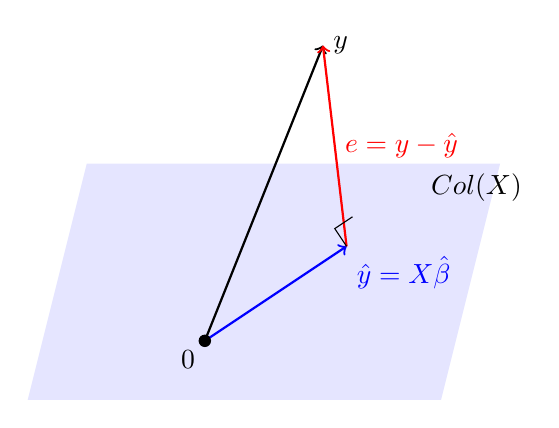
\begin{tikzpicture}[scale=1.5]
        % Draw the plane (column space)
        \fill[blue!10] (-1.5,-0.5) -- (2,-0.5) -- (2.5,1.5) -- (-1,1.5) -- cycle;
        \node at (2.3,1.3) {$\text{Col}(X)$};

        % Draw y vector
        \draw[->, thick] (0,0) -- (1,2.5) node[right] {$y$};

        % Draw y-hat (projection)
        \draw[->, thick, blue] (0,0) -- (1.2,0.8) node[below right] {$\hat{y} = X\hat{\beta}$};

        % Draw residual
        \draw[->, thick, red] (1.2,0.8) -- (1,2.5) node[midway, right] {$e = y - \hat{y}$};

        % Right angle marker
        \draw (1.2,0.8) -- (1.1,0.95) -- (1.25,1.05);

        % Origin
        \fill (0,0) circle (1.5pt) node[below left] {$0$};
    \end{tikzpicture}
    \caption{Geometric interpretation of OLS: $\hat{y}$ is the orthogonal projection of $y$ onto $\text{Col}(X)$, and the residual $e$ is perpendicular to the column space.}
\end{figure}

\begin{greybox}[Orthogonality of Residuals]
The residuals are orthogonal to the column space of $X$:
$$X^\top e = X^\top(y - X\hat{\beta}) = X^\top y - X^\top X (X^\top X)^{-1} X^\top y = X^\top y - X^\top y = 0$$

This is the \textbf{normal equations} in disguise: $X^\top(y - X\hat{\beta}) = 0$.

Geometrically: the error vector is perpendicular to the space of possible predictions. Each column of $X$ is orthogonal to $e$.
\end{greybox}

\begin{bluebox}[Why the Geometric View Matters]
The projection interpretation:
\begin{enumerate}
    \item \textbf{Explains uniqueness}: There is exactly one closest point in a subspace (assuming $X$ has full column rank)
    \item \textbf{Connects to Pythagoras}: $\|y\|^2 = \|\hat{y}\|^2 + \|e\|^2$-total variation splits into explained and unexplained. This is because $\hat{y}$ and $e$ are orthogonal.
    \item \textbf{Motivates $R^2$}: The coefficient of determination $R^2 = \|\hat{y} - \bar{y}\|^2 / \|y - \bar{y}\|^2$ measures how much of $y$'s variation lies in $\text{Col}(X)$
    \item \textbf{Generalises}: This view extends to ridge regression (regularised projection) and kernel methods
\end{enumerate}
\end{bluebox}

\subsection{What OLS Gives Us}

With $\hat{\beta} = (X^\top X)^{-1} X^\top y$, we can:

\begin{itemize}
    \item \textbf{Predict}: $\hat{y} = X\hat{\beta}$-fitted values for training data. For new data $x_{\text{new}}$, predict $\hat{y}_{\text{new}} = x_{\text{new}}^\top \hat{\beta}$.
    \item \textbf{Interpret}: $\hat{\beta}_j$ is the expected change in $y$ for a unit change in $x_j$, \emph{holding other features constant}. More precisely:
    $$\frac{\partial \hat{y}}{\partial x_j} = \hat{\beta}_j$$
    This ``ceteris paribus'' interpretation is crucial but often misunderstood-it's about partial derivatives, not total effects.
    \item \textbf{Quantify uncertainty}: Via $\text{Var}(\hat{\beta})$-how much would our estimates change with different data? This enables confidence intervals and hypothesis tests.
\end{itemize}

\section{KL Divergence and Cross-Entropy}

\begin{bluebox}[Section Summary]
KL divergence $D_{\text{KL}}(p \| q)$ measures how ``different'' distribution $q$ is from $p$. Intuition: the extra bits needed to encode samples from $p$ using a code optimised for $q$. Crucially asymmetric. Minimising KL divergence from data to model is equivalent to MLE.
\end{bluebox}

An alternative motivation for MLE comes from information theory: we want a model distribution $q_\theta$ that is ``close'' to the true data distribution $p$. But what does ``close'' mean for probability distributions? Ordinary Euclidean distance doesn't make sense for distributions. KL divergence provides the answer.

\subsection{Kullback-Leibler Divergence}

\begin{greybox}[Kullback-Leibler Divergence]
The KL divergence from $p$ to $q$ measures how much information is lost when $q$ is used to approximate $p$:

$$D_{\text{KL}}(p \| q) = \sum_{y} p(y) \log \frac{p(y)}{q(y)} = \mathbb{E}_{y \sim p}\left[\log \frac{p(y)}{q(y)}\right]$$

This can be decomposed as:
$$D_{\text{KL}}(p \| q) = \underbrace{-\sum_y p(y) \log p(y)}_{H(p) = \text{Entropy of } p} - \underbrace{\left(-\sum_y p(y) \log q(y)\right)}_{-H(p, q) = -\text{Cross-entropy}}$$

Rearranging: $D_{\text{KL}}(p \| q) = H(p, q) - H(p)$

For continuous distributions, replace sums with integrals:
$$D_{\text{KL}}(p \| q) = \int p(y) \log \frac{p(y)}{q(y)} \, dy$$

Properties:
\begin{itemize}
    \item $D_{\text{KL}}(p \| q) \geq 0$ (Gibbs' inequality)
    \item $D_{\text{KL}}(p \| q) = 0$ if and only if $p = q$
    \item \textbf{Not symmetric}: $D_{\text{KL}}(p \| q) \neq D_{\text{KL}}(q \| p)$ in general
\end{itemize}
\end{greybox}

\textbf{Unpacking the formula:} Let's understand what each part means:
\begin{itemize}
    \item $p(y)$ weights each outcome by its probability under the true distribution. We care more about getting common outcomes right than rare ones.
    \item $\log \frac{p(y)}{q(y)} = \log p(y) - \log q(y)$ compares the log-probability under $p$ versus $q$. If $q(y) < p(y)$, this term is positive-$q$ underestimates the probability of $y$.
    \item The expectation $\mathbb{E}_{y \sim p}[\cdot]$ averages over the true distribution $p$, not the model $q$.
\end{itemize}

\subsection{Information-Theoretic Intuition}

The KL divergence has a deep interpretation from coding theory that makes it more intuitive.

\textbf{Background}: To transmit data from a distribution $p$, the optimal code uses $-\log_2 p(y)$ bits for outcome $y$ (Shannon's source coding theorem). Common outcomes get short codes; rare outcomes get long codes. The expected code length is the \textbf{entropy} $H(p) = -\sum_y p(y) \log_2 p(y)$.

\textbf{The key insight}: If we use a code optimised for distribution $q$ but the data actually comes from $p$, we use $-\log q(y)$ bits for each outcome. The expected code length becomes the \textbf{cross-entropy} $H(p, q) = -\sum_y p(y) \log q(y)$.

\begin{bluebox}[KL Divergence as Extra Bits]
$$D_{\text{KL}}(p \| q) = H(p, q) - H(p) = \text{Expected extra bits needed}$$

KL divergence measures the \textbf{coding inefficiency}-how many extra bits we waste by using a code optimised for $q$ when the true distribution is $p$.

\textbf{Example}: If $p$ is uniform over 8 outcomes, the optimal code uses $\log_2(8) = 3$ bits per outcome. If we mistakenly use a code optimised for a different distribution $q$, we'll use more than 3 bits on average. The excess is $D_{\text{KL}}(p \| q)$.
\end{bluebox}

\subsection{Why Asymmetry Matters}

The asymmetry $D_{\text{KL}}(p \| q) \neq D_{\text{KL}}(q \| p)$ is not a defect but a feature with important consequences for machine learning.

\begin{greybox}[Asymmetry of KL Divergence]
Consider $p$ as the ``true'' distribution and $q$ as our model:

\textbf{Forward KL}: $D_{\text{KL}}(p \| q)$ - ``mean-seeking'' or ``moment-matching''
\begin{itemize}
    \item Penalises $q(y) \approx 0$ where $p(y) > 0$ (assigns low probability to likely events)
    \item The term $p(y) \log \frac{p(y)}{q(y)}$ explodes when $q(y) \to 0$ but $p(y) > 0$
    \item Forces $q$ to cover all modes of $p$-can't ignore any region where $p$ has mass
    \item Used in MLE: we average over the true data distribution
\end{itemize}

\textbf{Reverse KL}: $D_{\text{KL}}(q \| p)$ - ``mode-seeking''
\begin{itemize}
    \item Penalises $q(y) > 0$ where $p(y) \approx 0$ (assigns probability to unlikely events)
    \item OK to have $q(y) = 0$ where $p(y) > 0$ (ignoring some modes is acceptable)
    \item Allows $q$ to concentrate on one mode of $p$
    \item Used in variational inference: we average over the approximate distribution
\end{itemize}
\end{greybox}

\textbf{Visualising the asymmetry}: Let $p$ be a bimodal distribution (two peaks). A unimodal $q$ must choose:
\begin{itemize}
    \item \textbf{Forward KL} ($D_{\text{KL}}(p \| q)$): $q$ spreads to cover both modes, even if it assigns probability to the ``valley'' between them where $p$ has little mass.
    \item \textbf{Reverse KL} ($D_{\text{KL}}(q \| p)$): $q$ concentrates on one mode, ignoring the other entirely. This is acceptable because the penalty is proportional to $q(y)$, which is zero in the ignored region.
\end{itemize}

\begin{redbox}[Practical Implications of Asymmetry]
The choice of KL direction profoundly affects learned models:
\begin{itemize}
    \item \textbf{MLE} (forward KL) produces models that may be ``overconfident'' in regions between modes-assigning probability to outcomes that are actually unlikely under $p$
    \item \textbf{Variational inference} (reverse KL) may miss modes entirely, but is ``honest'' about uncertainty within the chosen mode
\end{itemize}
Understanding this asymmetry is essential for probabilistic modelling. Neither direction is ``correct''-the choice depends on what failure mode is more acceptable for your application.
\end{redbox}

\subsection{Cross-Entropy as a Loss Function}

\begin{greybox}[Cross-Entropy]
The cross-entropy between true distribution $p$ and model $q$:
$$H(p, q) = -\sum_y p(y) \log q(y)$$

For empirical data (where $p$ is the empirical distribution putting mass $1/n$ on each training example):
$$H(p_{\text{data}}, q_\theta) = -\frac{1}{n}\sum_{i=1}^n \log q_\theta(y_i)$$

This is exactly the NLL (up to a constant factor of $n$).
\end{greybox}

\begin{bluebox}[MLE Minimises KL Divergence]
Since the entropy of the true distribution $H(p)$ is constant (doesn't depend on model parameters), minimising KL divergence is equivalent to minimising cross-entropy:
$$\argmin_\theta D_{\text{KL}}(p \| q_\theta) = \argmin_\theta H(p, q_\theta) = \argmin_\theta \text{NLL}(\theta)$$

\textbf{Key insight}: MLE finds the model closest to the data in the KL sense. This gives MLE an information-theoretic justification beyond just ``maximising probability.''
\end{bluebox}

\section{Variance of the OLS Estimator}

\begin{bluebox}[Section Summary]
The OLS estimator $\hat{\beta}$ is unbiased with variance in ``sandwich form'': $\text{Var}(\hat{\beta}) = (X^\top X)^{-1} X^\top \mathbb{E}[\epsilon\epsilon^\top] X (X^\top X)^{-1}$. Under homoskedasticity this simplifies to $\sigma^2(X^\top X)^{-1}$. Robust standard errors handle heteroskedasticity by estimating the error covariance from residuals.
\end{bluebox}

To do inference (hypothesis tests, confidence intervals), we need the sampling distribution of $\hat{\beta}$. The key question: if we collected new data and recomputed $\hat{\beta}$, how much would it vary?

\subsection{Deriving the Variance}

Starting from $\hat{\beta} = (X^\top X)^{-1} X^\top y$ and substituting $y = X\beta + \epsilon$:

\begin{align*}
\hat{\beta} &= (X^\top X)^{-1} X^\top (X\beta + \epsilon) \\
&= (X^\top X)^{-1} X^\top X\beta + (X^\top X)^{-1} X^\top \epsilon \\
&= \beta + (X^\top X)^{-1} X^\top \epsilon
\end{align*}

This decomposition is illuminating: $\hat{\beta}$ equals the true $\beta$ plus a random perturbation $(X^\top X)^{-1} X^\top \epsilon$ that depends on the errors. The perturbation has mean zero (since $\mathbb{E}[\epsilon] = 0$), so $\hat{\beta}$ is unbiased.

\textbf{Unbiasedness}:
$$\mathbb{E}[\hat{\beta}] = \beta + (X^\top X)^{-1} X^\top \mathbb{E}[\epsilon] = \beta + 0 = \beta$$

So OLS is an \textbf{unbiased estimator}-on average, across many datasets, it gives the right answer.

\begin{greybox}[Sandwich Form of Variance]
\begin{align*}
\text{Var}(\hat{\beta}) &= \mathbb{E}[(\hat{\beta} - \beta)(\hat{\beta} - \beta)^\top] \\
&= \mathbb{E}[(X^\top X)^{-1} X^\top \epsilon \epsilon^\top X (X^\top X)^{-1}] \\
&= (X^\top X)^{-1} X^\top \mathbb{E}[\epsilon\epsilon^\top] X (X^\top X)^{-1}
\end{align*}

This is the \textbf{sandwich estimator}:
$$\text{Var}(\hat{\beta}) = \underbrace{(X^\top X)^{-1} X^\top}_{\text{bread}} \underbrace{\mathbb{E}[\epsilon\epsilon^\top]}_{\text{meat}} \underbrace{X (X^\top X)^{-1}}_{\text{bread}}$$
\end{greybox}

\textbf{Why ``sandwich''?} The covariance matrix of errors $\mathbb{E}[\epsilon\epsilon^\top]$ (the ``meat'') is sandwiched between two copies of $(X^\top X)^{-1}X^\top$ and its transpose (the ``bread''). This structure appears throughout statistics whenever we transform random variables by a linear operation.

The ``meat'' $\mathbb{E}[\epsilon\epsilon^\top]$ is the covariance matrix of the errors. Its structure depends on our assumptions about the error distribution.

\subsection{Homoskedastic Errors}

\begin{greybox}[Variance Under Homoskedasticity]
If errors have constant variance and are uncorrelated: $\mathbb{E}[\epsilon\epsilon^\top] = \sigma^2 I$

Then the sandwich simplifies dramatically:
\begin{align*}
\text{Var}(\hat{\beta}) &= (X^\top X)^{-1} X^\top \sigma^2 I \cdot X (X^\top X)^{-1} \\
&= \sigma^2 (X^\top X)^{-1} X^\top X (X^\top X)^{-1} \\
&= \sigma^2 (X^\top X)^{-1}
\end{align*}

The variance $\sigma^2$ is estimated by:
$$\hat{\sigma}^2 = \frac{1}{n-p} \sum_{i=1}^n (y_i - x_i^\top\hat{\beta})^2 = \frac{\text{RSS}}{n-p}$$

(We divide by $n-p$ rather than $n$ for unbiasedness-we ``used up'' $p$ degrees of freedom estimating $\beta$.)

The \textbf{standard error} of $\hat{\beta}_j$ is: $\text{SE}(\hat{\beta}_j) = \hat{\sigma}\sqrt{[(X^\top X)^{-1}]_{jj}}$
\end{greybox}

\textbf{Unpacking the homoskedasticity assumption}: The condition $\mathbb{E}[\epsilon\epsilon^\top] = \sigma^2 I$ means:
\begin{itemize}
    \item \textbf{Constant variance}: $\text{Var}(\epsilon_i) = \sigma^2$ for all $i$. The spread of errors is the same regardless of $x_i$.
    \item \textbf{Uncorrelated errors}: $\text{Cov}(\epsilon_i, \epsilon_j) = 0$ for $i \neq j$. Knowing one error tells us nothing about another.
\end{itemize}

\subsection{Heteroskedastic Errors}

When error variance varies across observations, the homoskedastic formula understates uncertainty for some coefficients and overstates it for others. We need \textbf{robust standard errors}.

\begin{greybox}[Heteroskedasticity-Consistent (HC) Standard Errors]
If $\text{Var}(\epsilon_i) = \sigma_i^2$ (varies with $i$), we can't simplify the sandwich. Instead, we estimate the meat directly:
$$\mathbb{E}[\epsilon\epsilon^\top] \approx \text{diag}(\hat{e}_1^2, \ldots, \hat{e}_n^2)$$
where $\hat{e}_i = y_i - x_i^\top\hat{\beta}$ are the residuals.

The \textbf{HC0 estimator} (White's robust standard errors):
$$\widehat{\text{Var}}(\hat{\beta}) = (X^\top X)^{-1} X^\top \text{diag}(\hat{e}^2) X (X^\top X)^{-1}$$

\textbf{To compute robust standard errors}:
\begin{enumerate}
    \item Calculate residuals: $\hat{e}_i = y_i - x_i^\top\hat{\beta}$
    \item Form the diagonal matrix $\Omega = \text{diag}(\hat{e}_1^2, \ldots, \hat{e}_n^2)$
    \item Compute the sandwich: $(X^\top X)^{-1} X^\top \Omega X (X^\top X)^{-1}$
    \item Take square roots of diagonal elements to get standard errors
\end{enumerate}
\end{greybox}

\begin{bluebox}[When to Use Robust Standard Errors]
\begin{itemize}
    \item \textbf{Always safe}: Robust SEs are valid under both homo- and heteroskedasticity
    \item \textbf{Efficiency}: If errors truly are homoskedastic, classical SEs are more efficient (lower variance)
    \item \textbf{Practice}: Many applied fields default to robust SEs as insurance
    \item \textbf{Individual variances}: Diagonal elements give variance of each $\hat{\beta}_j$; off-diagonals give covariances between coefficient estimates
\end{itemize}
\end{bluebox}

\begin{greybox}[Significance of the Variance of $\hat{\beta}$]
The variance-covariance matrix of $\hat{\beta}$ enables:
\begin{enumerate}
    \item \textbf{Statistical Significance}: Test whether coefficients differ from zero (or other values)
    \item \textbf{Confidence Intervals}: Quantify uncertainty in coefficient estimates
    \item \textbf{Precision Assessment}: Smaller variance = more precise estimates
    \item \textbf{Model Diagnostics}: High variance may indicate collinearity or insufficient data
    \item \textbf{Covariance Information}: Off-diagonal elements show how uncertainty in one coefficient relates to uncertainty in another
\end{enumerate}
\end{greybox}

\section{Bayesian Inference and MAP Estimation}

\begin{bluebox}[Section Summary]
Bayesian inference treats parameters as random variables with a prior $p(\theta)$. Bayes' rule combines prior and likelihood to give the posterior $p(\theta|\mathcal{D})$. MAP estimation finds the posterior mode; with Gaussian priors this yields Ridge regression, with Laplace priors it yields Lasso.
\end{bluebox}

MLE treats parameters as fixed unknowns. \textbf{Bayesian inference} treats parameters as random variables with distributions reflecting uncertainty. This is a fundamentally different philosophical stance with practical implications.

\begin{figure}[H]
    \centering
    \includegraphics[width=0.75\linewidth]{figures/week_02_training/image.png}
    \caption{Bayes' Rule: combining prior beliefs with observed data to form posterior beliefs. The posterior balances what we believed before (prior) with what the data tells us (likelihood).}
    \label{fig:bayes-rule}
\end{figure}

\begin{greybox}[Bayes' Rule for Parameter Inference]
$$p(\theta | \mathcal{D}) = \frac{p(\mathcal{D} | \theta) \cdot p(\theta)}{p(\mathcal{D})}$$

\begin{itemize}
    \item $p(\theta | \mathcal{D})$: \textbf{Posterior}-belief about $\theta$ after seeing data
    \item $p(\mathcal{D} | \theta)$: \textbf{Likelihood}-probability of data given parameters (same as MLE)
    \item $p(\theta)$: \textbf{Prior}-belief about $\theta$ before seeing data
    \item $p(\mathcal{D})$: \textbf{Marginal likelihood} (evidence)-normalising constant ensuring the posterior integrates to 1
\end{itemize}
\end{greybox}

\textbf{Unpacking Bayes' rule:}
\begin{itemize}
    \item The \textbf{prior} $p(\theta)$ encodes what we believe about the parameters before seeing any data. This could be informed by previous studies, domain knowledge, or simply a ``weakly informative'' default.
    \item The \textbf{likelihood} $p(\mathcal{D}|\theta)$ is exactly what MLE uses-the probability of the observed data under each possible parameter value.
    \item The \textbf{posterior} $p(\theta|\mathcal{D})$ combines both sources of information. It tells us what we should believe about $\theta$ after seeing the data.
    \item The \textbf{marginal likelihood} $p(\mathcal{D}) = \int p(\mathcal{D}|\theta) p(\theta) d\theta$ is a normalising constant. For point estimation (MAP), we can ignore it.
\end{itemize}

\begin{bluebox}[Frequentist vs Bayesian Perspectives]
\begin{center}
\begin{tabular}{l|l|l}
& \textbf{Frequentist (MLE)} & \textbf{Bayesian} \\
\hline
Parameters & Fixed, unknown constants & Random variables \\
Data & Random (from repeated sampling) & Fixed (what we observed) \\
Probability & Long-run frequency & Degree of belief \\
Primary quantity & $p(\mathcal{D}|\theta)$ (likelihood) & $p(\theta|\mathcal{D})$ (posterior) \\
\end{tabular}
\end{center}

\textbf{Objective probability} (frequentist): Based on facts about properties of the world. ``If we flip this coin infinitely many times, what fraction will be heads?''

\textbf{Subjective probability} (Bayesian): Based on our beliefs about the world. ``Given what I know, how confident am I that this coin is fair?''
\end{bluebox}

\subsection{Maximum A Posteriori (MAP) Estimation}

Full Bayesian inference requires computing the entire posterior distribution, which can be computationally demanding (often requiring Monte Carlo methods). MAP estimation finds just the \emph{mode} of the posterior-the single most probable parameter value.

\begin{greybox}[MAP Estimation]
$$\hat{\theta}_{\text{MAP}} = \argmax_\theta p(\theta | \mathcal{D}) = \argmax_\theta \frac{p(\mathcal{D}|\theta) \cdot p(\theta)}{p(\mathcal{D})}$$

Since $p(\mathcal{D})$ doesn't depend on $\theta$:
$$\hat{\theta}_{\text{MAP}} = \argmax_\theta \left[ p(\mathcal{D}|\theta) \cdot p(\theta) \right]$$

Taking logs (for computational convenience):
$$\hat{\theta}_{\text{MAP}} = \argmax_\theta \left[ \log p(\mathcal{D}|\theta) + \log p(\theta) \right]$$

This is MLE plus a \textbf{regularisation term} from the prior.
\end{greybox}

\textbf{The key insight}: MAP = MLE + Prior. The log-prior acts as a penalty term that discourages certain parameter values. Different priors give different penalties:

\begin{bluebox}[Connection Between MAP and Regularisation]
The choice of prior determines the type of regularisation:
\begin{itemize}
    \item \textbf{Gaussian prior}: $p(\theta) \propto \exp(-\lambda\|\theta\|_2^2)$ $\Rightarrow$ \textbf{Ridge regression} (L2 penalty)

    Taking logs: $\log p(\theta) = -\lambda\|\theta\|_2^2 + \text{const}$

    \item \textbf{Laplace prior}: $p(\theta) \propto \exp(-\lambda\|\theta\|_1)$ $\Rightarrow$ \textbf{Lasso} (L1 penalty)

    Taking logs: $\log p(\theta) = -\lambda\|\theta\|_1 + \text{const}$

    \item \textbf{Uniform/flat prior} (improper): $p(\theta) \propto 1$ $\Rightarrow$ MAP = MLE

    The log-prior is constant, so it doesn't affect the optimisation.
\end{itemize}
Regularisation isn't just a computational trick-it has a probabilistic interpretation as encoding prior beliefs about parameter values.
\end{bluebox}

\subsection{Interpreting Uncertainty: Credible vs Confidence Intervals}

With $\text{Var}(\hat{\beta})$, we can construct intervals. The interpretation differs fundamentally between paradigms:

\textbf{Bayesian (Credible Intervals)}:
\begin{itemize}
    \item Assume $\beta$ is random, data is fixed
    \item ``There is a 95\% probability that $\beta \in [l, u]$''
    \item Direct probability statement about the parameter
    \item Based on the posterior distribution $p(\beta|\mathcal{D})$
\end{itemize}

\textbf{Frequentist (Confidence Intervals)}:
\begin{itemize}
    \item Assume $\beta$ is fixed, data is random
    \item ``If we repeated this experiment many times, 95\% of the constructed intervals would contain the true $\beta$''
    \item Statement about the \emph{procedure}, not the parameter
    \item We don't assume a distribution for $\beta$; instead, we think about a process for constructing intervals
\end{itemize}

\begin{greybox}[Confidence Interval Construction]
$$[\hat{\beta} - z_{\alpha/2} \cdot \text{SE}(\hat{\beta}), \quad \hat{\beta} + z_{\alpha/2} \cdot \text{SE}(\hat{\beta})]$$

For 95\% confidence: $z_{0.025} \approx 1.96$

With finite samples and unknown $\sigma^2$, use $t$-distribution critical values instead:
$$[\hat{\beta} - t_{n-p, \alpha/2} \cdot \text{SE}(\hat{\beta}), \quad \hat{\beta} + t_{n-p, \alpha/2} \cdot \text{SE}(\hat{\beta})]$$
\end{greybox}

\begin{redbox}[Common Misinterpretation]
A 95\% confidence interval does \textbf{not} mean ``there is a 95\% probability that $\beta$ is in this interval.'' That's a Bayesian statement!

The frequentist statement is: ``The procedure that generated this interval has a 95\% success rate.'' The specific interval either contains $\beta$ or it doesn't-we just don't know which.

This distinction matters in practice: if you want to make probability statements about parameters, you need the Bayesian framework.
\end{redbox}

\section{Empirical Risk Minimisation}

\begin{bluebox}[Section Summary]
ERM generalises MLE: minimise average loss $\frac{1}{n}\sum_i \ell(y_i, f(x_i; \theta))$ over training data. Different losses suit different tasks. For classification, 0-1 loss is natural but non-convex; surrogate losses (log loss, hinge) are convex upper bounds that enable optimisation.
\end{bluebox}

MLE is one instance of a broader framework: \textbf{Empirical Risk Minimisation (ERM)}. The idea is simple: define a loss function that measures prediction error, then minimise the average loss on training data.

\begin{greybox}[Empirical Risk Minimisation]
Given a loss function $\ell(y, \hat{y})$ measuring prediction error:
$$\hat{\theta} = \argmin_\theta \frac{1}{n} \sum_{i=1}^n \ell(y_i, f(x_i; \theta))$$

This minimises the \textbf{empirical risk}-the average loss on training data.

Common loss functions include:
\begin{itemize}
    \item \textbf{NLL (for MLE)}: $\ell(y, \theta; x) = -\log p(y|x,\theta)$
    \item \textbf{Squared error}: $\ell(y, \hat{y}) = (y - \hat{y})^2$
    \item \textbf{0-1 loss}: $\ell(y, \hat{y}) = \mathbf{1}[y \neq \hat{y}]$
\end{itemize}
\end{greybox}

\textbf{Why ``empirical'' risk?} The true risk is the expected loss over the true data distribution: $R(\theta) = \mathbb{E}_{(x,y) \sim p}[\ell(y, f(x; \theta))]$. We can't compute this because we don't know $p$. The empirical risk approximates it using the training data as a sample from $p$.

\subsection{Common Loss Functions}

\begin{center}
\begin{tabular}{l|l|l}
\textbf{Loss} & \textbf{Formula} & \textbf{Use Case} \\
\hline
Squared (L2) & $(y - \hat{y})^2$ & Regression \\
Absolute (L1) & $|y - \hat{y}|$ & Robust regression \\
NLL (Gaussian) & $-\log p(y|\hat{y}, \sigma)$ & Probabilistic regression \\
0-1 Loss & $\mathbf{1}[y \neq \hat{y}]$ & Classification (ideal) \\
Log Loss (Cross-entropy) & $-y\log\hat{p} - (1-y)\log(1-\hat{p})$ & Probabilistic classification \\
Hinge Loss & $\max(0, 1 - y \cdot \hat{y})$ & SVM classification \\
\end{tabular}
\end{center}

\textbf{Why different losses?} Each loss encodes different priorities:
\begin{itemize}
    \item \textbf{L2 loss}: Penalises large errors heavily (squared). Sensitive to outliers.
    \item \textbf{L1 loss}: Penalises errors linearly. More robust to outliers.
    \item \textbf{0-1 loss}: Only cares about correct/incorrect, not confidence. The natural classification metric.
    \item \textbf{Log loss}: Rewards well-calibrated probability estimates. Penalises confident wrong predictions severely.
    \item \textbf{Hinge loss}: Focuses on margin-how far points are from the decision boundary.
\end{itemize}

\subsection{The Problem with 0-1 Loss}

\begin{redbox}[0-1 Loss is Intractable]
The \textbf{0-1 loss} (misclassification rate) is the natural classification loss-it directly measures what we care about. But it is:
\begin{itemize}
    \item \textbf{Non-convex}: Has many local minima; gradient descent may get stuck
    \item \textbf{Non-differentiable}: The function jumps from 0 to 1 at the decision boundary
    \item \textbf{Flat almost everywhere}: Gradient is zero except at decision boundary, providing no signal for optimisation
\end{itemize}

We cannot optimise it with gradient methods. Instead, we use \textbf{surrogate losses}.
\end{redbox}

\begin{figure}[H]
    \centering
    \includegraphics[width=0.75\linewidth]{figures/week_02_training/image_1.png}
    \caption{Surrogate loss functions compared to 0-1 loss. All surrogate losses upper bound the 0-1 loss while being differentiable and (mostly) convex.}
    \label{fig:surrogate-losses}
\end{figure}

\textbf{Surrogate losses} replace the 0-1 loss with something we can actually optimise. A good surrogate should:
\begin{enumerate}
    \item \textbf{Upper bound} the 0-1 loss: $\ell_{\text{surrogate}}(y, \hat{y}) \geq \mathbf{1}[y \neq \hat{y}]$. This ensures that minimising the surrogate also reduces misclassification.
    \item Be \textbf{convex}: Guarantees finding global minimum; no local minima traps.
    \item Be \textbf{differentiable}: Enables gradient-based optimisation.
    \item Be ``tight'': Close to 0-1 loss, so the approximation is good.
\end{enumerate}

\subsection{Classification Errors}

\begin{greybox}[Confusion Matrix]
\begin{center}
\begin{tabular}{cc|cc}
& & \multicolumn{2}{c}{\textbf{Predicted}} \\
& & Positive & Negative \\
\hline
\multirow{2}{*}{\textbf{Actual}} & Positive & TP (True Positive) & FN (False Negative) \\
& Negative & FP (False Positive) & TN (True Negative) \\
\end{tabular}
\end{center}

\begin{itemize}
    \item \textbf{Type I Error} (False Positive): Predict positive when actually negative. ``False alarm.''
    \item \textbf{Type II Error} (False Negative): Predict negative when actually positive. ``Missed detection.''
\end{itemize}
\end{greybox}

\begin{figure}[H]
    \centering
    \includegraphics[width=0.5\linewidth]{figures/week_02_training/image_2.png}
    \caption{Confusion matrix structure showing the four possible outcomes of binary classification.}
    \label{fig:confusion-matrix}
\end{figure}

Different applications weight these errors differently:
\begin{itemize}
    \item \textbf{Medical screening}: False negatives are dangerous (missing disease), so we tolerate more false positives. High \textbf{sensitivity} (recall) is prioritised.
    \item \textbf{Spam filtering}: False positives are annoying (good email marked as spam), so we tolerate more false negatives. High \textbf{precision} is prioritised.
    \item \textbf{Criminal justice}: ``Beyond reasonable doubt'' means we prefer false negatives (letting guilty go free) to false positives (convicting innocent).
\end{itemize}

\section{Convexity and Optimisation}

\begin{bluebox}[Section Summary]
Convex loss functions have a unique global minimum and no local minima traps. Gradient descent iteratively moves downhill in the loss landscape. For convex problems with appropriate step sizes, gradient descent is guaranteed to converge. Non-convex problems (neural networks) require more sophisticated approaches.
\end{bluebox}

When closed-form solutions don't exist (logistic regression, neural networks), we rely on iterative optimisation. The structure of the loss function determines how hard this is.

\subsection{Convex Functions}

\begin{greybox}[Convex Function]
A function $f: \mathbb{R}^d \to \mathbb{R}$ is \textbf{convex} if for all $x, y \in \mathbb{R}^d$ and $\lambda \in [0, 1]$:
$$f(\lambda x + (1-\lambda) y) \leq \lambda f(x) + (1-\lambda) f(y)$$

Geometrically: the line segment connecting any two points on the graph lies above (or on) the graph.

\textbf{Equivalent characterisations} (for twice-differentiable $f$):
\begin{itemize}
    \item First-order: $f(y) \geq f(x) + \nabla f(x)^\top (y - x)$ for all $x, y$

    (The tangent plane at any point lies below the function.)
    \item Second-order: $\nabla^2 f(x) \succeq 0$ for all $x$

    (The Hessian is positive semi-definite everywhere-the function curves upward.)
\end{itemize}
\end{greybox}

\textbf{Unpacking convexity}: The defining inequality says: if you take a weighted average of two inputs ($\lambda x + (1-\lambda)y$), the function value there is at most the weighted average of the function values ($\lambda f(x) + (1-\lambda)f(y)$). Visually, this means the function ``curves upward'' like a bowl.

\begin{bluebox}[Why Convexity Matters]
For convex functions:
\begin{enumerate}
    \item \textbf{Local = Global}: Any local minimum is a global minimum. No risk of getting stuck in suboptimal valleys.
    \item \textbf{Unique minimiser}: If the function is strictly convex (strict inequality), there is exactly one minimiser.
    \item \textbf{Guarantees}: We can prove convergence of optimisation algorithms.
    \item \textbf{Efficiency}: Polynomial-time algorithms exist for finding the minimum.
\end{enumerate}
\end{bluebox}

\textbf{Examples of convex losses}:
\begin{itemize}
    \item \textbf{Squared loss}: $(y - \hat{y})^2$-second derivative is $2 > 0$
    \item \textbf{Log loss}: $-y\log\hat{p} - (1-y)\log(1-\hat{p})$-can show Hessian is PSD
    \item \textbf{Hinge loss}: $\max(0, 1 - y \cdot \hat{y})$-convex but non-differentiable at the ``hinge''
\end{itemize}

\begin{redbox}[Non-Convexity in Deep Learning]
The 0-1 loss is \textbf{not convex}. Neither are neural network loss surfaces (due to nonlinear activations and the composition of many layers).

Deep learning succeeds despite non-convexity, but lacks the theoretical guarantees of convex optimisation. Current understanding suggests:
\begin{itemize}
    \item Many local minima exist, but they're often nearly as good as the global minimum
    \item Saddle points (not local minima) are the main obstacle
    \item Overparameterisation may help optimisation by creating more paths to good solutions
\end{itemize}
\end{redbox}

\subsection{Gradient Descent}

When no closed-form solution exists, we use iterative methods. Gradient descent is the workhorse of machine learning optimisation.

\begin{greybox}[Gradient Descent]
To minimise $\mathcal{L}(\theta)$, iterate:
$$\theta^{(t+1)} = \theta^{(t)} - \eta \nabla_\theta \mathcal{L}(\theta^{(t)})$$

where $\eta > 0$ is the \textbf{learning rate} (step size).

\textbf{Intuition}: The negative gradient $-\nabla \mathcal{L}$ points in the direction of steepest descent. We take a step of size $\eta$ in that direction.
\end{greybox}

\textbf{Geometric picture}: Imagine standing on a hilly landscape where height represents loss. The gradient tells you which way is uphill (steepest ascent). Gradient descent walks downhill, step by step, following the direction of steepest descent.

\textbf{Unpacking the update rule}:
\begin{itemize}
    \item $\nabla_\theta \mathcal{L}(\theta^{(t)})$ is the gradient-a vector pointing in the direction of steepest increase.
    \item The negative sign reverses this to point downhill.
    \item $\eta$ scales the step size. Too small: slow progress. Too large: overshoot and oscillate.
\end{itemize}

\begin{greybox}[Convergence for Convex Functions]
For a convex function $\mathcal{L}$ with \textbf{$L$-Lipschitz gradients} (i.e., $\|\nabla \mathcal{L}(x) - \nabla \mathcal{L}(y)\| \leq L\|x - y\|$):

With step size $\eta = 1/L$, gradient descent achieves:
$$\mathcal{L}(\theta^{(T)}) - \mathcal{L}(\theta^*) \leq \frac{L\|\theta^{(0)} - \theta^*\|^2}{2T}$$

This is $O(1/T)$ convergence: to get within $\epsilon$ of the optimum, we need $O(1/\epsilon)$ iterations.

For \textbf{strongly convex} functions (Hessian bounded below: $\nabla^2 \mathcal{L} \succeq \mu I$ for $\mu > 0$), convergence is exponentially faster: $O(\log(1/\epsilon))$ iterations.
\end{greybox}

\textbf{What is Lipschitz continuity of gradients?} It means the gradient doesn't change too rapidly. If the gradient changes slowly (small $L$), we can take larger steps safely. If it changes rapidly (large $L$), we need smaller steps to avoid overshooting.

\subsection{Choosing the Learning Rate}

\begin{bluebox}[Learning Rate Selection]
\begin{itemize}
    \item \textbf{Too small}: Slow convergence; may take forever to reach minimum
    \item \textbf{Too large}: Overshoots; may diverge (oscillate around minimum or explode)
    \item \textbf{Just right}: Fast, stable convergence
\end{itemize}

Rules of thumb:
\begin{itemize}
    \item Start with $\eta = 0.01$ or $0.001$
    \item Use learning rate schedules (decay over time): start large, decrease as you approach the minimum
    \item Adaptive methods (Adam, RMSprop) adjust per-parameter automatically
\end{itemize}
\end{bluebox}

\begin{figure}[H]
    \centering
    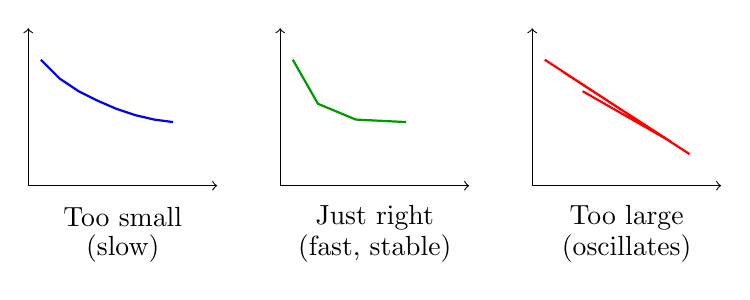
\begin{tikzpicture}[scale=0.8]
        % Too small
        \begin{scope}[xshift=-4cm]
            \draw[->] (0,0) -- (3,0);
            \draw[->] (0,0) -- (0,2.5);
            \draw[thick, blue] (0.2,2) -- (0.5,1.7) -- (0.8,1.5) -- (1.1,1.35) -- (1.4,1.22) -- (1.7,1.12) -- (2,1.05) -- (2.3,1.01);
            \node at (1.5,-0.5) {Too small};
            \node at (1.5,-1) {(slow)};
        \end{scope}

        % Just right
        \begin{scope}[xshift=0cm]
            \draw[->] (0,0) -- (3,0);
            \draw[->] (0,0) -- (0,2.5);
            \draw[thick, green!60!black] (0.2,2) -- (0.6,1.3) -- (1.2,1.05) -- (2,1.01);
            \node at (1.5,-0.5) {Just right};
            \node at (1.5,-1) {(fast, stable)};
        \end{scope}

        % Too large
        \begin{scope}[xshift=4cm]
            \draw[->] (0,0) -- (3,0);
            \draw[->] (0,0) -- (0,2.5);
            \draw[thick, red] (0.2,2) -- (2.5,0.5) -- (0.5,1.8) -- (2.2,0.7) -- (0.8,1.5);
            \node at (1.5,-0.5) {Too large};
            \node at (1.5,-1) {(oscillates)};
        \end{scope}
    \end{tikzpicture}
    \caption{Effect of learning rate on gradient descent convergence. Loss versus iteration for different learning rates.}
\end{figure}

\subsection{Stochastic Gradient Descent (SGD)}

For large datasets, computing the full gradient is expensive-it requires a pass through all $n$ samples.

\begin{greybox}[Stochastic Gradient Descent]
Instead of using all $n$ samples:
$$\nabla \mathcal{L}(\theta) = \frac{1}{n}\sum_{i=1}^n \nabla \ell_i(\theta)$$

Use a random \textbf{minibatch} $\mathcal{B} \subset \{1, \ldots, n\}$:
$$\nabla \mathcal{L}(\theta) \approx \frac{1}{|\mathcal{B}|}\sum_{i \in \mathcal{B}} \nabla \ell_i(\theta)$$

This is an unbiased estimate of the true gradient: $\mathbb{E}[\text{minibatch gradient}] = \text{full gradient}$.

The variance decreases with batch size: $\text{Var} \propto 1/|\mathcal{B}|$.
\end{greybox}

\begin{bluebox}[SGD Tradeoffs]
\begin{itemize}
    \item \textbf{Computation}: Each step is $O(|\mathcal{B}|)$ instead of $O(n)$-much faster per iteration
    \item \textbf{Noise}: Stochastic gradients are noisy estimates; updates are ``wiggly''
    \item \textbf{Regularisation}: Noise can help escape sharp minima (implicit regularisation)-may actually improve generalisation
    \item \textbf{Convergence}: More iterations needed, but much faster wall-clock time for large $n$
\end{itemize}

\textbf{Typical batch sizes}: 32, 64, 128, 256. Larger = more accurate gradients but slower per-epoch progress.
\end{bluebox}

\section{Logistic Regression}

\begin{bluebox}[Section Summary]
Logistic regression models $p(y=1|x) = \sigma(x^\top\beta)$ where $\sigma$ is the sigmoid. Trained by minimising binary cross-entropy (NLL for Bernoulli). No closed-form solution-requires iterative optimisation. Decision boundary is linear: the hyperplane $x^\top\beta = 0$.
\end{bluebox}

For binary classification, we need a model that outputs probabilities in $[0, 1]$. Linear regression won't work-it can produce any real number. We need a function that ``squashes'' the linear predictor into the valid probability range.

\begin{greybox}[Logistic Regression Model]
$$p(y = 1 | x, \beta) = \sigma(x^\top\beta) = \frac{1}{1 + e^{-x^\top\beta}}$$

where $\sigma(\cdot)$ is the \textbf{sigmoid} (logistic) function.

Equivalently, the observation follows a Bernoulli distribution:
$$y_i \sim \text{Bernoulli}(\sigma(x_i^\top\beta))$$

The \textbf{log-odds} (logit) is linear in the features:
$$\log \frac{p(y=1|x)}{p(y=0|x)} = \log \frac{p(y=1|x)}{1 - p(y=1|x)} = x^\top\beta$$
\end{greybox}

\textbf{Unpacking the model}:
\begin{itemize}
    \item $x^\top\beta$ is the linear predictor, same as in linear regression. It can be any real number.
    \item $\sigma(z) = \frac{1}{1 + e^{-z}}$ squashes this to $(0, 1)$. Large positive $z$ gives probability near 1; large negative $z$ gives probability near 0.
    \item The log-odds being linear means: each unit increase in $x_j$ adds $\beta_j$ to the log-odds of $y=1$.
\end{itemize}

\begin{figure}[H]
    \centering
    \includegraphics[width=0.75\linewidth]{figures/week_02_training/image_3.png}
    \caption{The sigmoid (logistic) function $\sigma(z) = 1/(1 + e^{-z})$ maps any real number to $(0, 1)$. At $z=0$, $\sigma(0) = 0.5$. The function saturates at 0 and 1 for large $|z|$.}
    \label{fig:sigmoid}
\end{figure}

The sigmoid function has useful properties:
\begin{itemize}
    \item \textbf{Range}: Maps $\mathbb{R} \to (0, 1)$-valid probabilities
    \item \textbf{Symmetric}: $\sigma(-z) = 1 - \sigma(z)$
    \item \textbf{Nice derivative}: $\sigma'(z) = \sigma(z)(1 - \sigma(z))$-easy to compute from the function value
    \item \textbf{Monotonic}: Larger $x^\top\beta$ means higher probability of $y=1$
\end{itemize}

\subsection{Training: Binary Cross-Entropy}

\begin{greybox}[Binary Cross-Entropy Loss]
The NLL for logistic regression (also called ``log loss'' or ``binary cross-entropy''):

Starting from the Bernoulli likelihood for one observation:
$$p(y_i | x_i, \beta) = \mu_i^{y_i} (1-\mu_i)^{1-y_i}$$

where $\mu_i = \sigma(x_i^\top\beta)$ and $y_i \in \{0, 1\}$.

Taking the negative log and averaging:
\begin{align*}
\text{NLL}(\beta) &= -\frac{1}{n} \sum_{i=1}^n \log\left[\mu_i^{y_i} (1-\mu_i)^{1-y_i}\right] \\
&= -\frac{1}{n} \sum_{i=1}^n \left[ y_i \log \mu_i + (1-y_i) \log(1-\mu_i) \right]
\end{align*}

\textbf{Gradient}:
$$\nabla_\beta \text{NLL} = \frac{1}{n} \sum_{i=1}^n (\mu_i - y_i) x_i = \frac{1}{n} X^\top (\mu - y)$$

This has the same form as linear regression's gradient! But $\mu$ depends nonlinearly on $\beta$ through the sigmoid.
\end{greybox}

\textbf{Unpacking the loss function}: For each observation:
\begin{itemize}
    \item If $y_i = 1$: loss is $-\log \mu_i$. We want $\mu_i$ (predicted probability of 1) to be high.
    \item If $y_i = 0$: loss is $-\log(1 - \mu_i)$. We want $\mu_i$ to be low (so $1-\mu_i$ is high).
\end{itemize}

The loss penalises confident wrong predictions severely: if $y_i = 1$ but $\mu_i \approx 0$, then $-\log \mu_i \to \infty$.

\begin{redbox}[No Closed-Form Solution]
Unlike linear regression, logistic regression has \textbf{no closed-form solution}. The dependence of $\mu_i$ on $\beta$ through the sigmoid makes the normal equations nonlinear. Setting the gradient to zero gives:
$$\sum_{i=1}^n (\sigma(x_i^\top\beta) - y_i) x_i = 0$$

This cannot be solved algebraically for $\beta$. We must use iterative optimisation:
\begin{itemize}
    \item \textbf{Gradient descent}: Simple but may be slow
    \item \textbf{Newton's method} (IRLS-Iteratively Reweighted Least Squares): Faster convergence using second derivatives
    \item \textbf{Quasi-Newton methods} (L-BFGS): Approximate Newton without computing full Hessian
\end{itemize}
\end{redbox}

\subsection{Decision Boundaries}

The classifier predicts $\hat{y} = 1$ when $p(y=1|x) > 0.5$. Since $\sigma(0) = 0.5$, this happens when $x^\top\beta > 0$.

\begin{bluebox}[Linear Decision Boundary]
The decision boundary $\{x : x^\top\beta = 0\}$ is a \textbf{hyperplane} in feature space.

\begin{itemize}
    \item In 2D (two features): the boundary is a line
    \item In 3D: a plane
    \item In general: a $(p-1)$-dimensional hyperplane in $p$-dimensional space
\end{itemize}

Logistic regression is a \textbf{linear classifier}-it can only separate classes with a linear boundary. For nonlinear boundaries, we need:
\begin{itemize}
    \item \textbf{Feature engineering}: Add polynomial features, interactions (e.g., $x_1^2$, $x_1 x_2$)
    \item \textbf{Kernel methods}: Implicitly map to high-dimensional feature space
    \item \textbf{Neural networks}: Learn nonlinear transformations of features
\end{itemize}
\end{bluebox}

\begin{figure}[H]
    \centering
    \includegraphics[width=0.75\linewidth]{figures/week_02_training/image_4.png}
    \caption{Linear decision boundary separating two classes. The boundary is the hyperplane where $x^\top\beta = 0$. Points on one side are classified as positive, points on the other as negative.}
    \label{fig:decision-boundary}
\end{figure}

\section{The Bias-Variance Tradeoff}

\begin{bluebox}[Section Summary]
Expected prediction error decomposes as $\text{MSE} = \text{Bias}^2 + \text{Variance} + \text{Irreducible noise}$. Simple models have high bias (systematic error), complex models have high variance (sensitivity to training data). Optimal model complexity balances both. This motivates regularisation.
\end{bluebox}

A fundamental tension in statistical learning: simple models underfit (high bias), complex models overfit (high variance). Understanding this tradeoff is crucial for building models that generalise well.

\begin{greybox}[Bias-Variance Decomposition for Estimators]
For an estimator $\hat{\theta}$ of true parameter $\theta$:

\textbf{Bias}: $\text{Bias}(\hat{\theta}) = \mathbb{E}[\hat{\theta}] - \theta$

How far is the average estimate from the truth? Measures \textbf{systematic error}.

\textbf{Variance}: $\text{Var}(\hat{\theta}) = \mathbb{E}[(\hat{\theta} - \mathbb{E}[\hat{\theta}])^2]$

How much does the estimate vary across different datasets? Measures \textbf{instability}.

\textbf{MSE Decomposition}:
$$\text{MSE}(\hat{\theta}) = \mathbb{E}[(\hat{\theta} - \theta)^2] = \text{Var}(\hat{\theta}) + \text{Bias}(\hat{\theta})^2$$
\end{greybox}

\subsection{Full Derivation of the Decomposition}

The MSE decomposition is fundamental. Let us derive it carefully using the ``add and subtract the mean'' trick.

\begin{greybox}[Derivation of Bias-Variance Decomposition]
Let $\bar{\theta} = \mathbb{E}[\hat{\theta}]$ denote the expected value of our estimator. We use the ``add and subtract'' trick:

\begin{align*}
\text{MSE}(\hat{\theta}) &= \mathbb{E}[(\hat{\theta} - \theta)^2] \\
&= \mathbb{E}[(\hat{\theta} - \bar{\theta} + \bar{\theta} - \theta)^2] \quad \text{(add and subtract $\bar{\theta}$)} \\
&= \mathbb{E}[(\hat{\theta} - \bar{\theta})^2 + 2(\hat{\theta} - \bar{\theta})(\bar{\theta} - \theta) + (\bar{\theta} - \theta)^2]
\end{align*}

Now we take expectations term by term:
\begin{itemize}
    \item \textbf{First term}: $\mathbb{E}[(\hat{\theta} - \bar{\theta})^2] = \text{Var}(\hat{\theta})$ by definition of variance
    \item \textbf{Second term}: $\mathbb{E}[2(\hat{\theta} - \bar{\theta})(\bar{\theta} - \theta)] = 2(\bar{\theta} - \theta)\mathbb{E}[\hat{\theta} - \bar{\theta}] = 2(\bar{\theta} - \theta) \cdot 0 = 0$

    This is zero because $\mathbb{E}[\hat{\theta}] = \bar{\theta}$ by definition, so $\mathbb{E}[\hat{\theta} - \bar{\theta}] = 0$.
    \item \textbf{Third term}: $\mathbb{E}[(\bar{\theta} - \theta)^2] = (\bar{\theta} - \theta)^2 = \text{Bias}(\hat{\theta})^2$

    This is a constant (not random), so expectation doesn't change it.
\end{itemize}

Therefore:
$$\boxed{\text{MSE}(\hat{\theta}) = \text{Var}(\hat{\theta}) + \text{Bias}(\hat{\theta})^2}$$
\end{greybox}

\subsection{Prediction Error Decomposition}

For prediction tasks, we decompose the expected prediction error at a test point $x_0$:

\begin{greybox}[Bias-Variance-Noise Decomposition for Prediction]
Assume the true model is $y = f(x) + \epsilon$ where $\epsilon \sim (0, \sigma^2)$ is irreducible noise. Let $\hat{f}(x)$ be our learned predictor (a random variable depending on training data).

The expected prediction error at $x_0$:
\begin{align*}
\mathbb{E}[(y_0 - \hat{f}(x_0))^2] &= \mathbb{E}[(f(x_0) + \epsilon - \hat{f}(x_0))^2] \\
&= \underbrace{\sigma^2}_{\text{irreducible}} + \underbrace{(f(x_0) - \mathbb{E}[\hat{f}(x_0)])^2}_{\text{bias}^2} + \underbrace{\mathbb{E}[(\hat{f}(x_0) - \mathbb{E}[\hat{f}(x_0)])^2]}_{\text{variance}}
\end{align*}

The expectation is over both the noise $\epsilon$ and the randomness in $\hat{f}$ from different training sets.
\end{greybox}

\textbf{The three components}:
\begin{enumerate}
    \item \textbf{Irreducible error} ($\sigma^2$): Noise inherent in the problem; cannot be reduced by any model, no matter how sophisticated. This is the ``floor'' on our prediction error.
    \item \textbf{Bias$^2$}: How far the average prediction is from the truth; measures systematic error. High bias means the model is ``too simple'' to capture the true relationship.
    \item \textbf{Variance}: How much predictions vary across different training sets; measures instability. High variance means the model is ``too complex'' and fits noise in the training data.
\end{enumerate}

\subsection{Visual Intuition: The Bullseye}

The bias-variance tradeoff has an intuitive interpretation as a target-shooting analogy:

\begin{center}
\begin{tabular}{c|c|c}
& \textbf{Low Variance} & \textbf{High Variance} \\
\hline
\textbf{Low Bias} & Tight cluster on bullseye & Scattered around bullseye \\
& \textit{(ideal)} & \textit{(overfitting)} \\
\hline
\textbf{High Bias} & Tight cluster off-centre & Scattered off-centre \\
& \textit{(underfitting)} & \textit{(worst case)} \\
\end{tabular}
\end{center}

\begin{itemize}
    \item \textbf{Bias} = how far the centre of mass of shots is from the bullseye
    \item \textbf{Variance} = how spread out the shots are around their centre of mass
    \item \textbf{MSE} = average squared distance from shots to bullseye = bias$^2$ + variance
\end{itemize}

\begin{bluebox}[The Tradeoff]
\begin{itemize}
    \item \textbf{Low bias, high variance}: Complex models (many parameters) fit training data well but vary wildly between samples-they \textbf{overfit}
    \item \textbf{High bias, low variance}: Simple models (few parameters) are stable but systematically wrong-they \textbf{underfit}
    \item \textbf{Optimal}: Balance that minimises total error (MSE = Bias$^2$ + Variance)
\end{itemize}

As model complexity increases: bias typically decreases, variance typically increases. There's a sweet spot in between.
\end{bluebox}

\subsection{Example: Shrinkage Estimators}

Consider estimating the mean $\mu$ of a normal distribution from $n$ samples $y_i \sim \mathcal{N}(\mu, \sigma^2)$.

\textbf{Sample mean}: $\bar{y} = \frac{1}{n}\sum_i y_i$
\begin{itemize}
    \item Unbiased: $\mathbb{E}[\bar{y}] = \mu$
    \item Variance: $\text{Var}(\bar{y}) = \sigma^2/n$
    \item MSE: $\sigma^2/n$ (since bias = 0)
\end{itemize}

\textbf{Shrinkage estimator}: $\tilde{y} = \frac{n}{n+k}\bar{y}$ (shrinks toward zero)
\begin{itemize}
    \item Biased: $\mathbb{E}[\tilde{y}] = \frac{n}{n+k}\mu \neq \mu$
    \item Lower variance: $\text{Var}(\tilde{y}) = \left(\frac{n}{n+k}\right)^2 \frac{\sigma^2}{n}$
\end{itemize}

\begin{greybox}[Bias-Variance Tradeoff in Shrinkage]
For the shrinkage estimator with parameter $k$:
\begin{itemize}
    \item \textbf{Bias}: $\mu - \frac{n}{n+k}\mu = \frac{k}{n+k}\mu$ (increases with $k$)
    \item \textbf{Variance}: $\left(\frac{n}{n+k}\right)^2 \frac{\sigma^2}{n}$ (decreases with $k$)
\end{itemize}

The parameter $k$ controls the compromise:
\begin{itemize}
    \item $k = 0$: No shrinkage, recover the unbiased sample mean
    \item Large $k$: Heavy shrinkage toward zero, low variance but high bias
\end{itemize}

When $|\mu|$ is small relative to $\sigma/\sqrt{n}$ (i.e., the true mean is close to our prior belief of zero), the variance reduction can outweigh the bias, giving lower MSE than the unbiased estimator.
\end{greybox}

This technique is useful when:
\begin{itemize}
    \item The sample size is small (high variance is a problem)
    \item There is substantial uncertainty about the sample mean
    \item We have prior information suggesting the parameter is near zero (or some other value)
\end{itemize}

\begin{bluebox}[Practical Implications]
\textbf{Unbiased is not always best.} If an unbiased estimator has high variance, a biased estimator with lower variance may have better overall performance (lower MSE). This insight motivates:
\begin{itemize}
    \item \textbf{Regularisation}: L1 (Lasso), L2 (Ridge) penalties shrink coefficients toward zero
    \item \textbf{Bayesian priors}: Encode beliefs that shrink estimates toward prior mean
    \item \textbf{Ensemble methods}: Averaging multiple models reduces variance
    \item \textbf{Early stopping}: Stop training before the model fully fits the training data
\end{itemize}
\end{bluebox}

\section{Preview: Regularisation and its Geometry}

\begin{bluebox}[Section Summary]
Regularisation adds a penalty to the loss function to control model complexity. L2 (Ridge) shrinks coefficients toward zero; L1 (Lasso) sets some coefficients exactly to zero. Geometrically, regularisation constrains the solution to lie within a region centred at the origin. Full treatment in Week 3.
\end{bluebox}

The bias-variance tradeoff motivates \textbf{regularisation}: intentionally introducing bias to reduce variance. We preview the geometric intuition here; detailed treatment follows in Week 3.

\subsection{Regularised Loss Functions}

\begin{greybox}[Regularised Objectives]
\textbf{Ridge Regression (L2 penalty)}:
$$\hat{\beta}_{\text{Ridge}} = \argmin_\beta \left\{ \|y - X\beta\|_2^2 + \lambda \|\beta\|_2^2 \right\}$$

\textbf{Lasso (L1 penalty)}:
$$\hat{\beta}_{\text{Lasso}} = \argmin_\beta \left\{ \|y - X\beta\|_2^2 + \lambda \|\beta\|_1 \right\}$$

The hyperparameter $\lambda \geq 0$ controls the strength of regularisation:
\begin{itemize}
    \item $\lambda = 0$: No regularisation, recover OLS
    \item $\lambda \to \infty$: Heavy regularisation, coefficients shrink to zero
\end{itemize}
\end{greybox}

\textbf{Unpacking the penalties}:
\begin{itemize}
    \item $\|\beta\|_2^2 = \sum_j \beta_j^2$ is the squared L2 norm-sum of squared coefficients
    \item $\|\beta\|_1 = \sum_j |\beta_j|$ is the L1 norm-sum of absolute values
\end{itemize}

Both penalties discourage large coefficients, but in different ways.

\subsection{Geometric Interpretation}

The regularised objective can be rewritten as a \textit{constrained} optimisation problem.

\begin{greybox}[Constrained Formulation]
By Lagrangian duality, Ridge regression is equivalent to:
$$\hat{\beta}_{\text{Ridge}} = \argmin_\beta \|y - X\beta\|_2^2 \quad \text{subject to} \quad \|\beta\|_2^2 \leq t$$

Similarly for Lasso with an L1 constraint: $\|\beta\|_1 \leq t$.

The Lagrange multiplier $\lambda$ and constraint bound $t$ are in one-to-one correspondence: larger $\lambda$ means smaller $t$.
\end{greybox}

\textbf{Geometric picture}:
\begin{itemize}
    \item The OLS solution $\hat{\beta}_{\text{OLS}}$ minimises the RSS. The contours of constant RSS are ellipses (in 2D) or ellipsoids (in higher dimensions) centred at $\hat{\beta}_{\text{OLS}}$.
    \item The constraint region is a ball (L2: $\|\beta\|_2 \leq t$) or diamond (L1: $\|\beta\|_1 \leq t$) centred at the origin.
    \item The regularised solution is where the RSS contours first touch the constraint region.
\end{itemize}

\begin{bluebox}[L1 vs L2: Sparsity]
\textbf{Why does L1 give sparse solutions?}

The L1 constraint region (a diamond/cross-polytope) has \textbf{corners} at the axes. Elliptical contours typically first touch the constraint at a corner, where some coordinates are exactly zero.

The L2 constraint region (a ball) is \textbf{smooth}. Contours touch it at a point where typically all coordinates are nonzero (just shrunk).

\textbf{Rule of thumb}:
\begin{itemize}
    \item \textbf{Ridge (L2)}: All coefficients shrunk, none exactly zero-good when all features are relevant
    \item \textbf{Lasso (L1)}: Some coefficients shrunk to exactly zero-performs feature selection
\end{itemize}
\end{bluebox}

\subsection{Ridge Regression: Closed Form}

Unlike Lasso, Ridge regression has an analytic solution.

\begin{greybox}[Ridge Solution]
$$\hat{\beta}_{\text{Ridge}} = (X^\top X + \lambda I)^{-1} X^\top y$$

Key properties:
\begin{itemize}
    \item \textbf{Always invertible}: Even when $X^\top X$ is singular, $X^\top X + \lambda I$ is invertible for $\lambda > 0$. The $\lambda I$ term ensures positive definiteness.
    \item \textbf{Shrinks toward zero}: As $\lambda$ increases, $\hat{\beta}_{\text{Ridge}} \to 0$
    \item \textbf{Bayesian interpretation}: Equivalent to posterior mean with Gaussian prior $\beta \sim \mathcal{N}(0, \sigma^2/\lambda \cdot I)$
\end{itemize}
\end{greybox}

\begin{bluebox}[Connection to Bias-Variance]
Regularisation trades bias for variance:
\begin{itemize}
    \item \textbf{Bias increases}: We're constraining $\beta$ away from the OLS solution
    \item \textbf{Variance decreases}: The constraint stabilises estimates against sampling variation
    \item \textbf{Optimal $\lambda$}: Chosen via cross-validation to minimise test error
\end{itemize}

This is the bias-variance tradeoff in action: we accept some systematic error (bias) in exchange for more stable predictions (lower variance).
\end{bluebox}

\section{Summary}

\begin{bluebox}[Key Concepts from Week 2]
\begin{enumerate}
    \item \textbf{MLE}: Choose parameters to maximise probability of observed data
    \item \textbf{NLL}: Negative log-likelihood-the loss function for MLE; minimising NLL = maximising likelihood
    \item \textbf{i.i.d.\ assumption}: Independence and identical distribution; substantively meaningful and often violated
    \item \textbf{Linear regression}: MLE with Gaussian errors $\Leftrightarrow$ least squares; justified by probabilistic assumptions
    \item \textbf{OLS solution}: $\hat{\beta} = (X^\top X)^{-1} X^\top y$ (orthogonal projection onto column space)
    \item \textbf{KL divergence}: Measures distribution ``distance''; MLE minimises $D_{\text{KL}}(p \| q)$
    \item \textbf{Variance of $\hat{\beta}$}: Sandwich form $(X^\top X)^{-1} X^\top \mathbb{E}[\epsilon\epsilon^\top] X (X^\top X)^{-1}$; simplifies under homoskedasticity
    \item \textbf{Robust SEs}: Handle heteroskedasticity via HC estimators
    \item \textbf{Bayesian inference}: Parameters as random variables; posterior = likelihood $\times$ prior
    \item \textbf{MAP}: MLE + prior = regularised estimation; Gaussian prior $\to$ Ridge, Laplace prior $\to$ Lasso
    \item \textbf{Convexity}: Guarantees global optimum; enables gradient descent convergence
    \item \textbf{Gradient descent}: Iterative optimisation; SGD scales to large data
    \item \textbf{Logistic regression}: Classification via sigmoid; trained with cross-entropy; no closed form
    \item \textbf{Bias-variance}: MSE = Bias$^2$ + Variance; tradeoff is fundamental
    \item \textbf{Regularisation}: L1/L2 penalties trade bias for variance; geometric constraint view
\end{enumerate}
\end{bluebox}

